\documentclass[16pt,fleqn]{article} % Default font size and left-justified equations

%----------------------------------------------------------------------------------------

%----------------------------------------------------------------------------------------
%	VARIOUS REQUIRED PACKAGES AND CONFIGURATIONS
%----------------------------------------------------------------------------------------

\usepackage[top=3cm,bottom=3cm,left=3cm,right=3cm,headsep=10pt,a4paper]{geometry} % Page margins

\usepackage{graphicx} % Required for including pictures
\graphicspath{{Pictures/}} % Specifies the directory where pictures are stored

\usepackage{lipsum} % Inserts dummy text
\usepackage{tikz} % Required for drawing custom shapes
\usepackage[final]{pdfpages}

\usepackage[english]{babel} % English language/hyphenation

\usepackage{enumitem} % Customize lists
\setlist{nolistsep} % Reduce spacing between bullet points and numbered lists

\usepackage{booktabs} % Required for nicer horizontal rules in tables

\usepackage{xcolor} % Required for specifying colors by name
\definecolor{ocre}{RGB}{84, 130, 53} %#548235

%----------------------------------------------------------------------------------------
%	FONTS
%----------------------------------------------------------------------------------------

\usepackage{avant} % Use the Avantgarde font for headings
%\usepackage{times} % Use the Times font for headings
\usepackage{mathptmx} % Use the Adobe Times Roman as the default text font together with math symbols from the Sym­bol, Chancery and Com­puter Modern fonts

\usepackage{microtype} % Slightly tweak font spacing for aesthetics
\usepackage[utf8]{inputenc} % Required for including letters with accents
\usepackage[T1]{fontenc} % Use 8-bit encoding that has 256 glyphs

%----------------------------------------------------------------------------------------
%	BIBLIOGRAPHY AND INDEX
%----------------------------------------------------------------------------------------

\usepackage[style=alphabetic,citestyle=numeric,sorting=nyt,sortcites=true,autopunct=true,babel=hyphen,hyperref=true,abbreviate=false,backref=true,backend=biber]{biblatex}
\addbibresource{bibliography.bib} % BibTeX bibliography file
\defbibheading{bibempty}{}

\usepackage{calc} % For simpler calculation - used for spacing the index letter headings correctly
\usepackage{makeidx} % Required to make an index
\makeindex % Tells LaTeX to create the files required for indexing

%----------------------------------------------------------------------------------------
%	MAIN TABLE OF CONTENTS
%----------------------------------------------------------------------------------------

\usepackage{titletoc} % Required for manipulating the table of contents

\contentsmargin{0cm} % Removes the default margin

% Part text styling
\titlecontents{part}[0cm]
{\addvspace{20pt}\centering\large\bfseries}
{}
{}
{}

% Chapter text styling
\titlecontents{chapter}[1.25cm] % Indentation
{\addvspace{12pt}\large\sffamily\bfseries} % Spacing and font options for chapters
{\color{ocre!60}\contentslabel[\Large\thecontentslabel]{1.25cm}\color{ocre}} % Chapter number
{\color{ocre}}  
{\color{ocre!60}\normalsize\;\titlerule*[.5pc]{.}\;\thecontentspage} % Page number

% Section text styling
\titlecontents{section}[1.25cm] % Indentation
{\addvspace{3pt}\sffamily\bfseries} % Spacing and font options for sections
{\contentslabel[\thecontentslabel]{1.25cm}} % Section number
{}
{\hfill\color{black}\thecontentspage} % Page number
[]

% Subsection text styling
\titlecontents{subsection}[1.25cm] % Indentation
{\addvspace{1pt}\sffamily\small} % Spacing and font options for subsections
{\contentslabel[\thecontentslabel]{1.25cm}} % Subsection number
{}
{\ \titlerule*[.5pc]{.}\;\thecontentspage} % Page number
[]

% List of figures
\titlecontents{figure}[0em]
{\addvspace{-5pt}\sffamily}
{\thecontentslabel\hspace*{1em}}
{}
{\ \titlerule*[.5pc]{.}\;\thecontentspage}
[]

% List of tables
\titlecontents{table}[0em]
{\addvspace{-5pt}\sffamily}
{\thecontentslabel\hspace*{1em}}
{}
{\ \titlerule*[.5pc]{.}\;\thecontentspage}
[]

%----------------------------------------------------------------------------------------
%	MINI TABLE OF CONTENTS IN PART HEADS
%----------------------------------------------------------------------------------------

% Chapter text styling
\titlecontents{lchapter}[0em] % Indenting
{\addvspace{15pt}\large\sffamily\bfseries} % Spacing and font options for chapters
{\color{ocre}\contentslabel[\Large\thecontentslabel]{1.25cm}\color{ocre}} % Chapter number
{}  
{\color{ocre}\normalsize\sffamily\bfseries\;\titlerule*[.5pc]{.}\;\thecontentspage} % Page number

% Section text styling
\titlecontents{lsection}[0em] % Indenting
{\sffamily\small} % Spacing and font options for sections
{\contentslabel[\thecontentslabel]{1.25cm}} % Section number
{}
{}

% Subsection text styling
\titlecontents{lsubsection}[.5em] % Indentation
{\normalfont\footnotesize\sffamily} % Font settings
{}
{}
{}

%----------------------------------------------------------------------------------------
%	THEOREM STYLES
%----------------------------------------------------------------------------------------

\usepackage{amsmath,amsfonts,amssymb,amsthm} % For math equations, theorems, symbols, etc

\newcommand{\intoo}[2]{\mathopen{]}#1\,;#2\mathclose{[}}
\newcommand{\ud}{\mathop{\mathrm{{}d}}\mathopen{}}
\newcommand{\intff}[2]{\mathopen{[}#1\,;#2\mathclose{]}}
\newtheorem{notation}{Notation}[section]

% Boxed/framed environments
\newtheoremstyle{ocrenumbox}% % Theorem style name
{0pt}% Space above
{0pt}% Space below
{\normalfont}% % Body font
{}% Indent amount
{\small\bf\sffamily\color{ocre}}% % Theorem head font
{\;}% Punctuation after theorem head
{0.25em}% Space after theorem head
{\small\sffamily\color{ocre}\thmname{#1}\nobreakspace\thmnumber{\@ifnotempty{#1}{}\@upn{#2}}% Theorem text (e.g. Theorem 2.1)
\thmnote{\nobreakspace\the\thm@notefont\sffamily\bfseries\color{black}---\nobreakspace#3.}} % Optional theorem note
\renewcommand{\qedsymbol}{$\blacksquare$}% Optional qed square

\newtheoremstyle{blacknumex}% Theorem style name
{5pt}% Space above
{5pt}% Space below
{\normalfont}% Body font
{} % Indent amount
{\small\bf\sffamily}% Theorem head font
{\;}% Punctuation after theorem head
{0.25em}% Space after theorem head
{\small\sffamily{\tiny\ensuremath{\blacksquare}}\nobreakspace\thmname{#1}\nobreakspace\thmnumber{\@ifnotempty{#1}{}\@upn{#2}}% Theorem text (e.g. Theorem 2.1)
\thmnote{\nobreakspace\the\thm@notefont\sffamily\bfseries---\nobreakspace#3.}}% Optional theorem note

\newtheoremstyle{blacknumbox} % Theorem style name
{0pt}% Space above
{0pt}% Space below
{\normalfont}% Body font
{}% Indent amount
{\small\bf\sffamily}% Theorem head font
{\;}% Punctuation after theorem head
{0.25em}% Space after theorem head
{\small\sffamily\thmname{#1}\nobreakspace\thmnumber{\@ifnotempty{#1}{}\@upn{#2}}% Theorem text (e.g. Theorem 2.1)
\thmnote{\nobreakspace\the\thm@notefont\sffamily\bfseries---\nobreakspace#3.}}% Optional theorem note

% Non-boxed/non-framed environments
\newtheoremstyle{ocrenum}% % Theorem style name
{5pt}% Space above
{5pt}% Space below
{\normalfont}% % Body font
{}% Indent amount
{\small\bf\sffamily\color{ocre}}% % Theorem head font
{\;}% Punctuation after theorem head
{0.25em}% Space after theorem head
{\small\sffamily\color{ocre}\thmname{#1}\nobreakspace\thmnumber{\@ifnotempty{#1}{}\@upn{#2}}% Theorem text (e.g. Theorem 2.1)
\thmnote{\nobreakspace\the\thm@notefont\sffamily\bfseries\color{black}---\nobreakspace#3.}} % Optional theorem note
\renewcommand{\qedsymbol}{$\blacksquare$}% Optional qed square
\makeatother

% Defines the theorem text style for each type of theorem to one of the three styles above
\newcounter{dummy} 
\numberwithin{dummy}{section}
\theoremstyle{ocrenumbox}
\newtheorem{theoremeT}[dummy]{Theorem}
\newtheorem{problem}{Problem}[section]
\newtheorem{exerciseT}{Exercise}[section]
\theoremstyle{blacknumex}
\newtheorem{exampleT}{Example}[section]
\theoremstyle{blacknumbox}
\newtheorem{vocabulary}{Vocabulary}[section]
\newtheorem{definitionT}{Definition}[section]
\newtheorem{corollaryT}[dummy]{Corollary}
\newtheorem{fonctionT}[dummy]{fonction}
\theoremstyle{ocrenum}
\newtheorem{proposition}[dummy]{Proposition}

%----------------------------------------------------------------------------------------
%	DEFINITION OF COLORED BOXES
%----------------------------------------------------------------------------------------

\RequirePackage[framemethod=default]{mdframed} % Required for creating the theorem, definition, exercise and corollary boxes

% Theorem box
\newmdenv[skipabove=7pt,
skipbelow=7pt,
backgroundcolor=black!5,
linecolor=ocre,
innerleftmargin=5pt,
innerrightmargin=5pt,
innertopmargin=5pt,
leftmargin=0cm,
rightmargin=0cm,
innerbottommargin=5pt]{tBox}

% Exercise box	  
\newmdenv[skipabove=7pt,
skipbelow=7pt,
rightline=false,
leftline=true,
topline=false,
bottomline=false,
backgroundcolor=ocre!10,
linecolor=ocre,
innerleftmargin=5pt,
innerrightmargin=5pt,
innertopmargin=5pt,
innerbottommargin=5pt,
leftmargin=0cm,
rightmargin=0cm,
linewidth=4pt]{eBox}	

% Definition box
\newmdenv[skipabove=7pt,
skipbelow=7pt,
rightline=false,
leftline=true,
topline=false,
bottomline=false,
linecolor=ocre,
innerleftmargin=5pt,
innerrightmargin=5pt,
innertopmargin=0pt,
leftmargin=0cm,
rightmargin=0cm,
linewidth=4pt,
innerbottommargin=0pt]{dBox}	

% Corollary box
\newmdenv[skipabove=7pt,
skipbelow=7pt,
rightline=false,
leftline=true,
topline=false,
bottomline=false,
linecolor=gray,
backgroundcolor=black!5,
innerleftmargin=5pt,
innerrightmargin=5pt,
innertopmargin=5pt,
leftmargin=0cm,
rightmargin=0cm,
linewidth=4pt,
innerbottommargin=5pt]{cBox}

% Fonction box
\newmdenv[skipabove=7pt,
skipbelow=7pt,
rightline=false,
leftline=true,
topline=false,
bottomline=false,
linecolor=ocre,
backgroundcolor=black!5,
innerleftmargin=5pt,
innerrightmargin=5pt,
innertopmargin=5pt,
leftmargin=0cm,
rightmargin=0cm,
linewidth=4pt,
innerbottommargin=5pt]{fBox}

% Creates an environment for each type of theorem and assigns it a theorem text style from the "Theorem Styles" section above and a colored box from above
\newenvironment{theorem}{\begin{tBox}\begin{theoremeT}}{\end{theoremeT}\end{tBox}}
\newenvironment{exercise}{\begin{eBox}\begin{exerciseT}}{\hfill{\color{ocre}\tiny\ensuremath{\blacksquare}}\end{exerciseT}\end{eBox}}				  
\newenvironment{definition}{\begin{dBox}\begin{definitionT}}{\end{definitionT}\end{dBox}}	
\newenvironment{example}{\begin{exampleT}}{\hfill{\tiny\ensuremath{\blacksquare}}\end{exampleT}}		
\newenvironment{corollary}{\begin{cBox}\begin{corollaryT}}{\end{corollaryT}\end{cBox}}	
\newenvironment{fonction}{\begin{cBox}\begin{fonctionT}}{\end{fonctionT}\end{fBox}}	

%----------------------------------------------------------------------------------------
%	REMARK ENVIRONMENT
%----------------------------------------------------------------------------------------

\newenvironment{remark}{\par\vspace{10pt}\small % Vertical white space above the remark and smaller font size
\begin{list}{}{
\leftmargin=35pt % Indentation on the left
\rightmargin=25pt}\item\ignorespaces % Indentation on the right
\makebox[-2.5pt]{
\begin{tikzpicture}[overlay]
\node[draw=ocre!60,line width=1pt,circle,fill=ocre!25,font=\sffamily\bfseries,inner sep=2pt,outer sep=0pt] at (-15pt,0pt){\textcolor{ocre}{R}};\end{tikzpicture}} % Orange R in a circle
\advance\baselineskip -1pt}{\end{list}\vskip5pt} % Tighter line spacing and white space after remark

%----------------------------------------------------------------------------------------
%	SECTION NUMBERING IN THE MARGIN
%----------------------------------------------------------------------------------------

\makeatletter
\renewcommand{\@seccntformat}[1]{\llap{\textcolor{ocre}{\csname the#1\endcsname}\hspace{1em}}}                    
\renewcommand{\section}{\@startsection{section}{1}{\z@}
{-4ex \@plus -1ex \@minus -.4ex}
{1ex \@plus.2ex }
{\normalfont\large\sffamily\bfseries}}
\renewcommand{\subsection}{\@startsection {subsection}{2}{\z@}
{-3ex \@plus -0.1ex \@minus -.4ex}
{0.5ex \@plus.2ex }
{\normalfont\sffamily\bfseries}}
\renewcommand{\subsubsection}{\@startsection {subsubsection}{3}{\z@}
{-2ex \@plus -0.1ex \@minus -.2ex}
{.2ex \@plus.2ex }
{\normalfont\small\sffamily\bfseries}}                        
\renewcommand\paragraph{\@startsection{paragraph}{4}{\z@}
{-2ex \@plus-.2ex \@minus .2ex}
{.1ex}
{\normalfont\small\sffamily\bfseries}}

%----------------------------------------------------------------------------------------
%	PART HEADINGS
%----------------------------------------------------------------------------------------

% numbered part in the table of contents
\newcommand{\@mypartnumtocformat}[2]{%
\setlength\fboxsep{0pt}%
\noindent\colorbox{ocre!20}{\strut\parbox[c][.7cm]{\ecart}{\color{ocre!70}\Large\sffamily\bfseries\centering#1}}\hskip\esp\colorbox{ocre!40}{\strut\parbox[c][.7cm]{\linewidth-\ecart-\esp}{\Large\sffamily\centering#2}}}%
%%%%%%%%%%%%%%%%%%%%%%%%%%%%%%%%%%
% unnumbered part in the table of contents
\newcommand{\@myparttocformat}[1]{%
\setlength\fboxsep{0pt}%
\noindent\colorbox{ocre!40}{\strut\parbox[c][.7cm]{\linewidth}{\Large\sffamily\centering#1}}}%
%%%%%%%%%%%%%%%%%%%%%%%%%%%%%%%%%%
\newlength\esp
\setlength\esp{4pt}
\newlength\ecart
\setlength\ecart{1.2cm-\esp}
\newcommand{\thepartimage}{}%
\newcommand{\partimage}[1]{\renewcommand{\thepartimage}{#1}}%
\def\@part[#1]#2{%
\ifnum \c@secnumdepth >-2\relax%
\refstepcounter{part}%
\addcontentsline{toc}{part}{\texorpdfstring{\protect\@mypartnumtocformat{\thepart}{#1}}{\partname~\thepart\ ---\ #1}}
\else%
\addcontentsline{toc}{part}{\texorpdfstring{\protect\@myparttocformat{#1}}{#1}}%
\fi%
\startcontents%
\markboth{}{}%
{\thispagestyle{empty}%
\begin{tikzpicture}[remember picture,overlay]%
\node at (current page.north west){\begin{tikzpicture}[remember picture,overlay]%	
\fill[ocre!20](0cm,0cm) rectangle (\paperwidth,-\paperheight);
\node[anchor=north] at (4cm,-3.25cm){\color{ocre!40}\fontsize{220}{100}\sffamily\bfseries\thepart}; 
\node[anchor=south east] at (\paperwidth-1cm,-\paperheight+1cm){\parbox[t][][t]{8.5cm}{
\printcontents{l}{0}{\setcounter{tocdepth}{1}}%
}};
\node[anchor=north east] at (\paperwidth-1.5cm,-3.25cm){\parbox[t][][t]{15cm}{\strut\raggedleft\color{white}\fontsize{30}{30}\sffamily\bfseries#2}};
\end{tikzpicture}};
\end{tikzpicture}}%
\@endpart}
\def\@spart#1{%
\startcontents%
\phantomsection
{\thispagestyle{empty}%
\begin{tikzpicture}[remember picture,overlay]%
\node at (current page.north west){\begin{tikzpicture}[remember picture,overlay]%	
\fill[ocre!20](0cm,0cm) rectangle (\paperwidth,-\paperheight);
\node[anchor=north east] at (\paperwidth-1.5cm,-3.25cm){\parbox[t][][t]{15cm}{\strut\raggedleft\color{white}\fontsize{30}{30}\sffamily\bfseries#1}};
\end{tikzpicture}};
\end{tikzpicture}}
\addcontentsline{toc}{part}{\texorpdfstring{%
\setlength\fboxsep{0pt}%
\noindent\protect\colorbox{ocre!40}{\strut\protect\parbox[c][.7cm]{\linewidth}{\Large\sffamily\protect\centering #1\quad\mbox{}}}}{#1}}%
\@endpart}
\def\@endpart{\vfil\newpage
\if@twoside
\if@openright
\null
\thispagestyle{empty}%
\newpage
\fi
\fi
\if@tempswa
\twocolumn
\fi}

%----------------------------------------------------------------------------------------
%	CHAPTER HEADINGS
%----------------------------------------------------------------------------------------

% A switch to conditionally include a picture, implemented by  Christian Hupfer
\newif\ifusechapterimage
\usechapterimagetrue
\newcommand{\thechapterimage}{}%
\newcommand{\chapterimage}[1]{\ifusechapterimage\renewcommand{\thechapterimage}{#1}\fi}%
\newcommand{\autodot}{.}
\def\@makechapterhead#1{%
{\parindent \z@ \raggedright \normalfont
\ifnum \c@secnumdepth >\m@ne
\if@mainmatter
\begin{tikzpicture}[remember picture,overlay]
\node at (current page.north west)
{\begin{tikzpicture}[remember picture,overlay]
\node[anchor=north west,inner sep=0pt] at (0,0) {\ifusechapterimage\includegraphics[width=\paperwidth]{\thechapterimage}\fi};
\draw[anchor=west] (\Gm@lmargin,-5cm) node [line width=2pt,rounded corners=15pt,draw=ocre,fill=white,fill opacity=0.5,inner sep=15pt]{\strut\makebox[22cm]{}};
\draw[anchor=west] (\Gm@lmargin+.3cm,-5cm) node {\huge\sffamily\bfseries\color{black}\thechapter\autodot~#1\strut};
\end{tikzpicture}};
\end{tikzpicture}
\else
\begin{tikzpicture}[remember picture,overlay]
\node at (current page.north west)
{\begin{tikzpicture}[remember picture,overlay]
\node[anchor=north west,inner sep=0pt] at (0,0) {\ifusechapterimage\includegraphics[width=\paperwidth]{\thechapterimage}\fi};
\draw[anchor=west] (\Gm@lmargin,-9cm) node [line width=2pt,rounded corners=15pt,draw=ocre,fill=white,fill opacity=0.5,inner sep=15pt]{\strut\makebox[22cm]{}};
\draw[anchor=west] (\Gm@lmargin+.3cm,-9cm) node {\huge\sffamily\bfseries\color{black}#1\strut};
\end{tikzpicture}};
\end{tikzpicture}
\fi\fi\par\vspace*{150\p@}}}

%-------------------------------------------

\def\@makeschapterhead#1{%
\begin{tikzpicture}[remember picture,overlay]
\node at (current page.north west)
{\begin{tikzpicture}[remember picture,overlay]
\node[anchor=north west,inner sep=0pt] at (0,0) {\ifusechapterimage\includegraphics[width=\paperwidth]{\thechapterimage}\fi};
\draw[anchor=west] (\Gm@lmargin,-5cm) node [line width=2pt,rounded corners=15pt,draw=ocre,fill=white,fill opacity=0.5,inner sep=15pt]{\strut\makebox[22cm]{}};
\draw[anchor=west] (\Gm@lmargin+.3cm,-5cm) node {\huge\sffamily\bfseries\color{black}#1\strut};
\end{tikzpicture}};
\end{tikzpicture}
\par\vspace*{150\p@}}
\makeatother

%----------------------------------------------------------------------------------------
%	HYPERLINKS IN THE DOCUMENTS
%----------------------------------------------------------------------------------------

\usepackage{hyperref}
\hypersetup{hidelinks,backref=true,pagebackref=true,hyperindex=true,colorlinks=false,breaklinks=true,urlcolor= ocre,bookmarks=true,bookmarksopen=false,pdftitle={Title},pdfauthor={Author}}
\usepackage{bookmark}
\bookmarksetup{
open,
numbered,
addtohook={%
\ifnum\bookmarkget{level}=0 % chapter
\bookmarksetup{bold}%
\fi
\ifnum\bookmarkget{level}=-1 % part
\bookmarksetup{color=ocre,bold}%
\fi
}
}

\usepackage[explicit]{titlesec}
\AtBeginEnvironment{align}{\setcounter{equation}{0}}
\usepackage{chngcntr}
\counterwithout{equation}{section}
\usepackage{longtable}
\usepackage{tabu}
\usepackage{xcolor,colortbl}
\usepackage{hhline}
\usepackage{listings}

\usepackage{eso-pic,graphicx,transparent}
\newcommand{\bgimg}[1]{
\AddToShipoutPicture
   {
      \put(\LenToUnit{-3.5cm},\LenToUnit{-1cm})
      {
            {\transparent{0.13}\includegraphics[width=25.3cm,height=32cm]{#1}}
      }
   }
} % Insert the commands.tex file which contains the majority of the structure behind the template

\begin{document}


%----------------------------------------------------------------------------------------
%	COPYRIGHT PAGE
%----------------------------------------------------------------------------------------
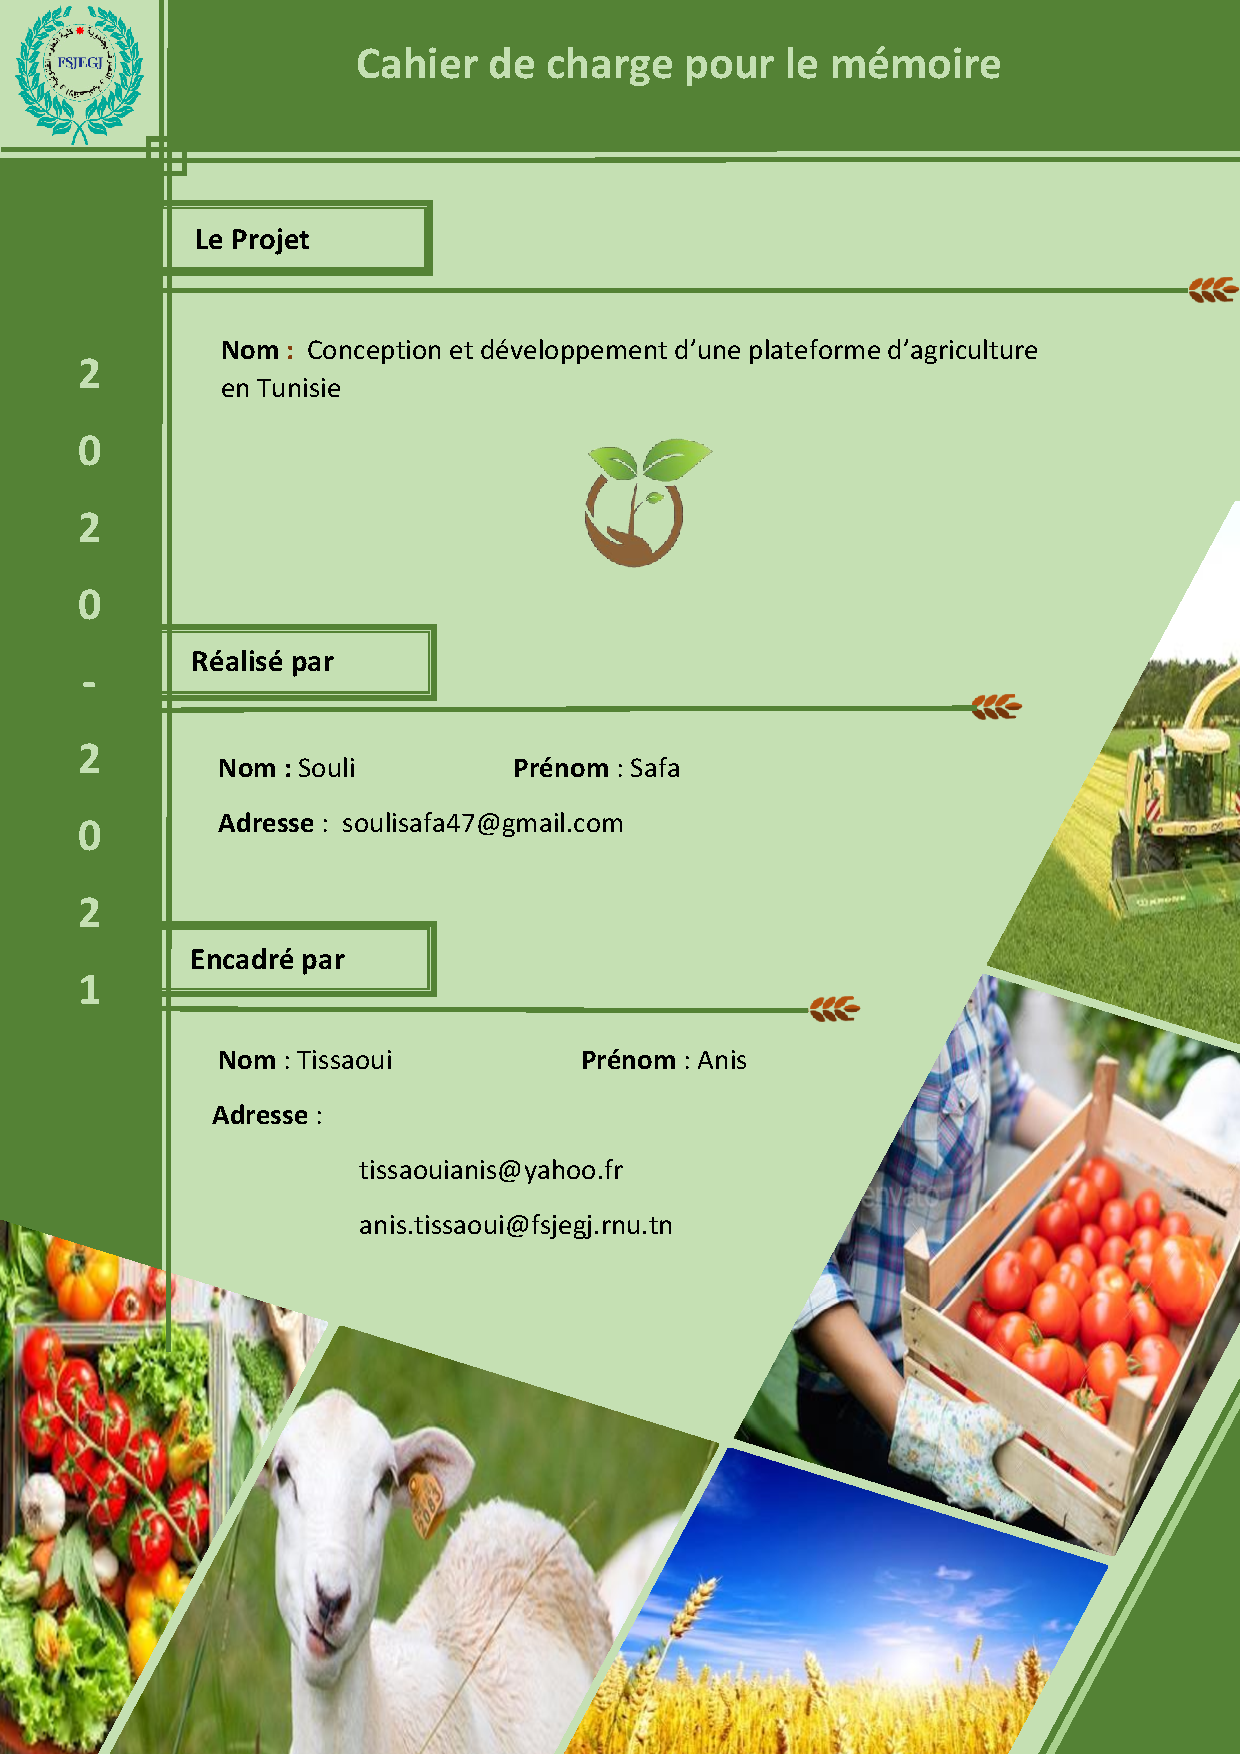
\includepdf[pages=-]{cover.pdf}
\bgimg{Pictures/border.png} % met une image de fond sour toutes les pages à partir d'ici

\section{Contexte et définition du problème}

Dans cette vie réelle, nous allons découvrir de nouvelles idées qui nous rendent la vie plus facile que par le passé et automatique. Donc, dans ce cas, nous avons travaillé dans le domaine agricole, dans ce domaine la plupart des gens ont des problèmes avec les aliments frais de la ferme que nous avons eu des fraudes.
Il y a aussi une pénurie de matières premières pour l'agriculture comme le lait, le poisson, le poulet, les œufs, etc.

\section{Objectif du projet}
Nous voulons offrir un meilleur service dans nos réponses aux clients à l'aide d'un outil de l'inter-médiation entre le fermes et les clients. Aujourd'hui le taux de satisfaction est à 60\%, nous visons les 80\% un an après la mise en place du nouvel outil.

\section{Périmètre}
Nous concentrons sur les clients de la nord de la Tunisie, avec domaine de plateforme : www.freshnat.com.tn.

\section{Acteur}
\tabulinesep = 3mm
\noindent
\begin{longtabu} to \textwidth {|[3pt,ocre]|[1pt,ocre]c|[ocre]X[5mm]|[1pt,ocre]|[3pt,ocre]}
    \caption{Définition des acteurs}\\
    \arrayrulecolor{ocre}
    \hhline{|=|=|}
        \color{ocre}\textbf{Acteur} & \color{ocre}\textbf{Définition}\\
        \hhline{|=|=|}
    Agriculteur & C'est l'acteur qui peut vendre ces produits aux clients. \\\hline
    Client & C'est l'acteur qui peut acheter des produits d'un agriculteur en ligne par commande. \\\hline
    Livreur & C'est l'acteur qui livre les commandes aux clients. \\\hline
    Système & C'est l'acteur utilisé pour recommandation les produit et les agriculteurs \\\hline
   Administrateur & C'est l'acteur qui gère tous.\\\hhline{|=|=|}
\end{longtabu}

\section{Description fonctionnelle des besoins}
Notre plateforme Centré autour de quatre acteurs:


\subsection{Client}
Les fonctionnalités de cet acteur sont :
\subsubsection{Gérer d'accès}
\begin{itemize}
    \item \textbf{S'authentifier :} Où lequel peut accéder à son espace privé de plateforme après l'inscription.
    \item \textbf{S'inscrire :} Où lequel peut créer son espace privé de plateforme pour accéder.
    \item \textbf{Confirmer mail :} Où lequel peut confirmer son mail.
    \item \textbf{Réinitialiser mot de passe :} Où lequel peut créer un nouveau mot de passe après une confirmation de compte.
\end{itemize}
\subsubsection{Mise à jour profil :}
\begin{itemize}
    \item \textbf{Modifier profil :} Où lequel peut modifier ses informations de son compte.
    \item \textbf{Supprimer profil :} Où lequel peut supprimer son compte.
\end{itemize}

\subsubsection{Consulter ferme :}
Où lequel peut consulter les détails de ferme.

\subsubsection{Gérer avis :}
\begin{itemize}
    \item \textbf{Consulter avis :} Où lequel peut consulter les avis des produits.
    \item \textbf{Donner avis :} Où lequel peut donner un avis d'une ferme.
    \item \textbf{Modifier avis :} Où lequel peut modifier son avis sur une ferme.
    \item \textbf{Supprimer avis :} Où lequel peut supprimer son avis sur une ferme.
\end{itemize}

\subsubsection{Consulter produit :}
Où lequel peut consulter des produit d'une ferme.

\subsubsection{Gérer note :}
\begin{itemize}
    \item \textbf{Noter produit :} Où lequel peut donner une note comprise entre 1 et 5 sur un produit d'une ferme.
    \item \textbf{Consulter note :} Où lequel peut consulter les notes des produits.
    \item \textbf{Annuler note :} Où lequel peut annuler sa note.
\end{itemize}

\subsubsection{Consulter catégorie :}
Où lequel peut consulter les produits par catégorie.

\subsubsection{Gérer panier :}
    \begin{itemize}
        \item \textbf{Consulter panier :} Où lequel peut consulter liste des produit ajouté récemment au panier.
        \item \textbf{Ajouter produit au panier :} Où lequel peut ajouter un produit au son panier.
        \item \textbf{Supprimer produit du panier :} Où lequel peut modifier les quantités des produits de son panier.
    \end{itemize}
    
\subsubsection{Gérer commande :}
    \begin{itemize}
        \item \textbf{Commander produit :} Où lequel peut commander des produit ajouté récemment au panier.
        \item \textbf{Annuler commande :} Où lequel peut annuler sa commande.
        \item \textbf{Suivre commande :} Où lequel peut suivre si la commande est en attende, en cours ou préparée.
    \end{itemize}
    
\subsubsection{Gérer livraison :}
Où lequel peut suivre la livraison de sa commande est déjà confirmé
\begin{itemize}
        \item \textbf{Suivre livraison :} Où lequel peut suivre la livraison de sa commande est déjà confirmé
        \item \textbf{Demande livraison :} Où lequel peut envoyer une demande de livraison au livreur.
    \end{itemize}

\subsubsection{Gérer forum :}
    \begin{itemize}
        \item \textbf{Consulter forum :} Où lequel peut consulter un forum.
        \item \textbf{Ajouter forum :} Où lequel peut ajouter un forum.
        \item \textbf{Modifier forum :} Où lequel peut modifier son forum.
        \item \textbf{Supprimer forum :} Où lequel peut supprimer son forum.
    \end{itemize}
    
\subsubsection{Gérer commentaire :}
    \begin{itemize}
        \item \textbf{Commenter forum :} Où lequel peut commenter sur un forum.
        \item \textbf{consulter commentaire :} Où lequel peut consulter les commentaires sur un forum.
        \item \textbf{Modifier commentaire :} Où lequel peut modifier son commentaire sur un forum.
        \item \textbf{Supprimer commentaire :} Où lequel peut supprimer son commentaire d'un forum.
    \end{itemize}
    
\subsubsection{Gérer répondre :}
    \begin{itemize}
        \item \textbf{Répondre commentaire :} Où lequel peut commenter sur un forum.
        \item \textbf{Consulter répondre :} Où lequel peut modifier son commentaire sur un forum.
        \item \textbf{Modifier répondre :} Où lequel peut modifier son commentaire sur un forum.
        \item \textbf{Supprimer répondre :} Où lequel peut supprimer son commentaire d'un forum.
    \end{itemize}  
    
\subsubsection{Gérer paiement :}
    \begin{itemize}
        \item \textbf{Choisir mode de paiement :} Où lequel peut choisir mode de paiement (Chèque, Carte Bancaire, Paypal ou Espèce).
        \item \textbf{Payer commande:} Où lequel peut modifier son commentaire sur un forum.
    \end{itemize}
    
\subsection{Agriculteur}
Les fonctionnalités de cet acteur sont :
\subsubsection{Gérer d'accès}
\begin{itemize}
    \item \textbf{S'authentifier :} Où lequel peut accéder à son espace privé de plateforme après l'inscription.
    \item \textbf{Demande d'inscrire :} Où lequel peut demander d'être un agriculteur
    \item \textbf{Réinitialiser mot de passe :} Où lequel peut créer un nouveau mot de passe après une confirmation de compte.
\end{itemize}
\subsubsection{Mise à jour profil :}
\begin{itemize}
    \item \textbf{Modifier profil :} Où lequel peut modifier ses informations de son compte.
    \item \textbf{Demander suppression profil :} Où lequel peut envoyer demande au administrateur pour supprimer son compte.
\end{itemize}

\subsubsection{Gérer ferme :}
\begin{itemize}
    \item \textbf{Consulter ferme :} Où lequel peut consulter des fermes.
    \item \textbf{Ajouter ferme :} Où lequel peut ajouter une ferme.
    \item \textbf{Modifier ferme :} Où lequel peut modifier sa ferme.
    \item \textbf{Supprimer ferme :} Où lequel peut supprimer sa ferme.
\end{itemize}
\subsubsection{Consulter avis :}
Où lequel peut consulter les avis d'une ferme.

\subsubsection{Gérer produit :}
\begin{itemize}
    \item \textbf{Consulter produit :} Où lequel peut consulter les produits des fermes.
    \item \textbf{Ajouter produit :} Où lequel peut ajouter un produit au son ferme.
    \item \textbf{Modifier produit :} Où lequel peut modifier les informations d'un produit ajoutées par lui.
    \item \textbf{Supprimer produit :} Où lequel peut supprimer un produit de son ferme.
\end{itemize}

\subsubsection{Gérer note :}
\begin{itemize}
    \item \textbf{Noter produit :} Où lequel peut donner une note comprise entre 1 et 5 sur un produit d'une ferme.
    \item \textbf{Consulter note :} Où lequel peut consulter les notes des produits.
    \item \textbf{Annuler note :} Où lequel peut annuler sa note.
\end{itemize}

\subsubsection{Consulter catégorie :}
Où lequel peut consulter les produits par catégorie.
    
\subsubsection{Gérer commande :}
    \begin{itemize}
        \item \textbf{Consulter commande :} Où lequel peut consulter les commandes de son ferme.
        \item \textbf{Préparer commande :} Où lequel peut accepter, refuser ou mettre en cours une commande.
        \item \textbf{Supprimer commande :} Où lequel peut supprimer les commandes de sa ferme.
    \end{itemize}
    
\subsubsection{Suivre livraison :}
Où lequel peut suivre le livreur pour arrive à sa ferme.

\subsubsection{Gérer forum :}
    \begin{itemize}
        \item \textbf{Consulter forum :} Où lequel peut consulter un forum.
        \item \textbf{Ajouter forum :} Où lequel peut ajouter un forum.
        \item \textbf{Modifier forum :} Où lequel peut modifier son forum.
        \item \textbf{Supprimer forum :} Où lequel peut supprimer son forum.
    \end{itemize}
    
\subsubsection{Gérer commentaire :}
    \begin{itemize}
        \item \textbf{Commenter forum :} Où lequel peut commenter sur un forum.
        \item \textbf{Consulter commentaire :} Où lequel peut consulter les commentaires des forums.
        \item \textbf{Modifier commentaire :} Où lequel peut modifier son commentaire sur un forum.
        \item \textbf{Supprimer commentaire :} Où lequel peut supprimer son commentaire d'un forum.
    \end{itemize}
    
\subsubsection{Gérer répondre :}
    \begin{itemize}
        \item \textbf{Répondre commentaire :} Où lequel peut commenter sur un forum.
        \item \textbf{Consulter répondre :} Où lequel peut consulter les  répondes des commentaires des forums.
        \item \textbf{Modifier répondre :} Où lequel peut modifier son commentaire sur un forum.
        \item \textbf{Supprimer répondre :} Où lequel peut supprimer son commentaire d'un forum.
    \end{itemize}  

\subsection{Livreur}
Les fonctionnalités de cet acteur sont :
\subsubsection{Gérer d'accès}
\begin{itemize}
    \item \textbf{S'authentifier :} Où lequel peut accéder à son espace privé de plateforme après l'inscription.
    \item \textbf{Demande d'inscrire :} Où lequel peut demander d'être un agriculteur
    \item \textbf{Confirmer mail :} Où lequel peut confirmer son mail.
    \item \textbf{Réinitialiser mot de passe :} Où lequel peut créer un nouveau mot de passe après une confirmation de compte.
\end{itemize}
\subsubsection{Mise à jour profil :}
\begin{itemize}
    \item \textbf{Modifier profil :} Où lequel peut modifier ses informations de son compte.
    \item \textbf{Demander suppression profil :} Où lequel peut envoyer demande au administrateur pour supprimer son compte.
\end{itemize}

\subsubsection{Consulter ferme :}
Où lequel peut consulter les détails de ferme.

\subsubsection{Gérer avis :}
\begin{itemize}
    \item \textbf{Donner avis :} Où lequel peut donner un avis d'une ferme.
    \item \textbf{Consulter avis :} Où lequel peut consulter des avis de fermes.
    \item \textbf{Modifier avis :} Où lequel peut modifier son avis sur une ferme.
    \item \textbf{Supprimer avis :} Où lequel peut supprimer son avis sur une ferme.
\end{itemize}

\subsubsection{Consulter produit :}
Où lequel peut consulter des produit d'une ferme.

\subsubsection{Gérer note :}
\begin{itemize}
    \item \textbf{Noter produit :} Où lequel peut donner une note comprise entre 1 et 5 sur un produit d'une ferme.
    \item \textbf{Annuler note :} Où lequel peut annuler sa note.
\end{itemize}

\subsubsection{Consulter catégorie :}
Où lequel peut consulter les produits par catégorie.

\subsubsection{Gérer panier :}
    \begin{itemize}
        \item \textbf{Consulter panier :} Où lequel peut consulter son panier.
        \item \textbf{Ajouter produit au panier :} Où lequel peut ajouter un produit au son panier.
        \item \textbf{Modifier panier :} Où lequel peut modifier les quantités des produits de son panier.
        \item \textbf{Supprimer produit de panier :} Où lequel peut supprimer des produits de son panier.
    \end{itemize}
    
\subsubsection{Gérer commande :}
    \begin{itemize}
        \item \textbf{Commander produit :} Où lequel peut commander des produit ajouté récemment au panier.
        \item \textbf{Consulter commande :} Où lequel peut consulter sa commande.
        \item \textbf{Annuler commande :} Où lequel peut annuler sa commande.
        \item \textbf{Suivre commande :} Où lequel peut suivre si la commande est en attende, en cours ou préparée.
    \end{itemize}
    
\subsubsection{Gérer livraison :}
    \begin{itemize}
        \item \textbf{Consulter livraison :} Où lequel peut consulter une livraison.
        \item \textbf{Traiter livraison :} Où lequel peut accepter, refusé, mettre en cours une demande de livraison ou changer ligne de transport.
        \item \textbf{annuler livraison :} Où lequel peut annuler une livraison.
    \end{itemize}
    
\subsubsection{Gérer forum :}
    \begin{itemize}
        \item \textbf{Consulter forum :} Où lequel peut consulter des forums.
        \item \textbf{Ajouter forum :} Où lequel peut ajouter un forum.
        \item \textbf{Modifier forum :} Où lequel peut modifier son forum.
        \item \textbf{Supprimer forum :} Où lequel peut supprimer son forum.
    \end{itemize}
    
\subsubsection{Gérer commentaire :}
    \begin{itemize}
        \item \textbf{Commenter forum :} Où lequel peut commenter sur un forum.
        \item \textbf{Consulter commentaire :} Où lequel peut consulter des commentaires de forums.
        \item \textbf{Modifier commentaire :} Où lequel peut modifier son commentaire sur un forum.
        \item \textbf{Supprimer commentaire :} Où lequel peut supprimer son commentaire d'un forum.
    \end{itemize}
    
\subsubsection{Gérer répondre :}
    \begin{itemize}
        \item \textbf{Répondre commentaire :} Où lequel peut commenter sur un forum.
        \item \textbf{Consulter répondre :} Où lequel peut consulter les répondes de commentaires sur un forum.
        \item \textbf{Modifier répondre :} Où lequel peut modifier son commentaire sur un forum.
        \item \textbf{Supprimer répondre :} Où lequel peut supprimer son commentaire d'un forum.
    \end{itemize}  
    
\subsection{Système}
Les fonctionnalités de cet acteur sont :
\subsubsection{Gérer recommandation}
\begin{itemize}
    \item  \textbf{Recommander agriculteur : }
    Où lequel recommander des agriculteurs aux clients ou visiteurs.
    \item  \textbf{Recommander produit : }
    Où lequel recommander des produits aux clients ou visiteurs.
    \item  \textbf{Recommander livreur : }
    Où lequel recommander des livreurs aux clients ou visiteurs.
\end{itemize}

\subsection{Administrateur}

Les fonctionnalités de cet acteur sont :

\subsubsection{Gérer demande d'inscription:}
\begin{itemize}
    \item \textbf{Accepter demande :} Où lequel peut accepter les demandes d'inscription des agriculteurs ou des livreurs.
    \item \textbf{Refusé demande :} Où lequel peut refuser les demandes d'inscription des agriculteurs ou des livreurs.
\end{itemize}
\subsubsection{Gérer demande de suppression:}
\begin{itemize}
    \item \textbf{Accepter demande :} Où lequel peut accepter les demandes de suppression des comptes des agriculteurs ou des livreurs.
    \item \textbf{Refuser demande :} Où lequel peut refuser les demandes de suppression des comptes des agriculteurs ou des livreurs.
\end{itemize}


\subsubsection{Gérer catégorie :}
Où lequel peut consulter les produits par catégorie.
    \begin{itemize}
        \item \textbf{Consulter catégorie :} Où lequel peut Consulter des catégories de produits.
        \item \textbf{Ajouter catégorie :} Où lequel peut ajouter une catégorie de produits.
        \item \textbf{Modifier catégorie :} Où lequel peut modifier une catégorie de produits.
        \item \textbf{Supprimer catégorie :} Où lequel peut supprimer une catégorie de produits.
    \end{itemize}
    
\subsection{Délais}
\end{document}
